\documentclass[11pt]{article}
\usepackage[a4paper,margin=1in]{geometry}
\usepackage{amsmath,amssymb,amsthm,mathtools}
\usepackage[expansion=false]{microtype}
\usepackage{graphicx,booktabs,array}
\usepackage[font=small,labelfont=bf]{caption}
\usepackage[dvipsnames]{xcolor}
\usepackage{enumitem}
\usepackage[hidelinks,pdfusetitle]{hyperref}
\usepackage[nameinlink,capitalise]{cleveref}
\setlist{nosep,leftmargin=1.5em}
\newtheorem{theorem}{Theorem}[section]
\newtheorem{lemma}[theorem]{Lemma}
\newtheorem{proposition}[theorem]{Proposition}
\newtheorem{corollary}[theorem]{Corollary}
\newtheorem{conjecture}{Conjecture}
\theoremstyle{definition}\newtheorem{definition}[theorem]{Definition}
\theoremstyle{remark}\newtheorem{remark}[theorem]{Remark}
\newcommand{\R}{\mathbb R}\newcommand{\C}{\mathbb C}\newcommand{\N}{\mathbb N}
\newcommand{\dd}{\,\mathrm d}\newcommand{\e}{\mathrm e}
\renewcommand{\Re}{\operatorname{Re}}\renewcommand{\Im}{\operatorname{Im}}
\newcommand{\fr}[1]{\{#1\}}
\setlength{\parskip}{0.35em}
\AtBeginDocument{\sloppy}
\urlstyle{same}
\hypersetup{pdftitle={The Balance of the Count: One Energy in the Prime Counts and in the Sawtooth},pdfauthor={Abhijit Singh}}
\title{\textbf{The Balance of the Count:}\\[4pt]
\large One Energy in the Prime Counts and in the Sawtooth, and the Riemann Hypothesis in Real Variables}
\author{Abhijit Singh}
\date{26 September 2026}
\begin{document}
\maketitle
\begin{abstract}
We write the Riemann Hypothesis (RH) in real variables and measure the constant it predicts in three independent ways, which agree to within $2\%$. Every integer $k>1$ has as many squarefree divisors with an even number of prime factors as with an odd number, and this pairing gives the rebuild law $\sum_{n\le x}M(x/n)=1$ for the Mertens function $M$: the balance at every scale is fixed by the balances at all smaller scales. We prove that the Möbius-weighted sawtooths rebuild the constant exactly, $-\sum_{k\ge1}\mu(k)\fr{1/(kt)}=\chi_{(0,1]}(t)$ for every $t>0$, and that the first $N$ of them fall short by a value term $x\,m(N)$, $m(N)=\sum_{k\le N}\mu(k)/k$, and by a signed sum $R_N(x)$ of the unfinished divisor sums $c_N(n)$ over $N<n\le x$; the integral of the squared shortfall over $[1/N,1]$ is exactly $(N-1)\,m(N)^2$, which does not tend to $0$. We prove that RH is equivalent to the statement that the energy $E(X)=\int_1^X((\psi(x)-x)/x)^2\dd x$ of the prime-count error grows more slowly than every power of $X$. Measured in doublings $u=\log_2x$, the error of the prime counts to $10^{10}$ shows real waves at $1.560$, $2.320$, $2.760$, $3.358$, $3.633$, $4.148$, $4.515$ and $4.780$ turns per doubling; each wave grows by $2^{u(1/2+\delta)}$ with $|\delta|\le0.0022$ between the two halves of the range, and the first wave's amplitude in the two halves agrees to $0.4\%$. The mean energy per unit of $\log x$ is $0.04592$ over $2^{12}\le x\le10^{10}$, and $0.04587$ and $0.04597$ in the two halves. The sum $\sum1/|\rho|^2$ over the zeros with $|\gamma|<3000$ ($2469$ conjugate pairs), with the density tail, is $0.046192$, and the sawtooth distance of Nyman, Beurling and B\'aez-Duarte, computed from exact integrals of fractional parts with no reference to primes, gives $d_N^2\log N$ between $0.0454$ and $0.0470$ for $40\le N\le60$; all three agree with $2+\gamma-\log4\pi=0.0461914$ to within $2\%$. The rebuild law, with a table of $\mu$ to $10^9$, reproduces $M(10^n)$ exactly for $9\le n\le15$ and gives $|M(x)|\le0.424\sqrt x$ at every doubling from $2^{34}$ to $2^{49}$. The integers free of the primes up to $37$ carry no wave (amplitude at most $0.0018$ against $0.14$--$0.18$), while at $x=10^{10}$ the Möbius sum over the integers whose prime factors are at most $x/2$ is $+2200.6\sqrt x$ and the primes in $(x/2,x]$ bring it to $M(x)=-0.337\sqrt x$. Generalized-integer systems of Diamond, Montgomery and Vorhauer and of Broucke, Debruyne and R\'ev\'esz obey the same pairing and the same rebuild law, the latter with integer-count error $O(x^{1/2+\varepsilon})$, and have prime errors far above $\sqrt x$; a proof of RH must therefore use more about the integer count than these properties, and the ordinary count has more: it is exact, $\lfloor x\rfloor=x-\fr x$ with $0\le\fr x<1$. We state the remaining step as the subpolynomial growth of the energy.
\end{abstract}

\tableofcontents

\section{Introduction}\label{sec:intro}

Let $\mu$ be the Möbius function, $M(x)=\sum_{n\le x}\mu(n)$ the Mertens function, $\Lambda$ the von Mangoldt function and $\psi(x)=\sum_{n\le x}\Lambda(n)$. The Riemann Hypothesis (RH) is the conjecture that every nontrivial zero $\rho=\beta+i\gamma$ of $\zeta$ has $\beta=\frac12$. Littlewood proved that RH is equivalent to $M(x)\ll x^{1/2+\varepsilon}$ for every $\varepsilon>0$ \cite[\S14.25]{Titchmarsh}, and von Koch proved that under RH $\psi(x)-x\ll\sqrt x\log^2x$ \cite{vonKoch}. Both statements compare a count with a balanced walk: a walk of $n$ independent steps $\pm1$ has mean square $n$, because every cross term $s_is_j$ is cancelled by its opposite, and so spreads as $\sqrt n$. RH says that the Möbius sign $\mu(n)$, the parity of the number of prime factors of a squarefree $n$, summed over the integers, spreads no faster than such a walk, up to $x^\varepsilon$.

The main criterion (\cref{mt:energy}) and every measurement in this paper are stated in real variables. The zeros of $\zeta$ enter the measurements only through the real waves they produce in the counts, each wave being described by two real numbers, its growth exponent $\beta$ and its pitch, and the constants $\pi$ and $\e$ enter only as units: we measure $x$ in doublings, $u=\log_2x$, and pitch in turns per doubling.

\subsection{Main results}

\begin{theorem}[pair cancellation and the rebuild law]\label{mt:rebuild}
\begin{enumerate}[label=\textup{(\roman*)}]
\item For every integer $k>1$, $\sum_{d\mid k}\mu(d)=0$: the squarefree divisors of $k$ fall into pairs $\{d,dp\}$, $p\mid k$ a fixed prime, with $\mu(dp)=-\mu(d)$.
\item For every real $x\ge1$, $\sum_{n\le x}M(x/n)=1$.
\item $M$ is the only function $F$ on $(0,\infty)$ with $F=0$ on $(0,1)$ and $\sum_{n\le x}F(x/n)=1$ for all $x\ge1$.
\end{enumerate}
\end{theorem}

The law determines the balance at every scale from the balances at smaller scales. The next theorem splits a sum of dilated sawtooths into a value part and a count part.

\begin{theorem}[count and value of the sawtooth sum]\label{mt:countvalue}
For an integer $N\ge1$ and real $x\ge1$ let $m(N)=\sum_{k\le N}\mu(k)/k$, $c_N(n)=\sum_{k\mid n,\,k\le N}\mu(k)$ and $R_N(x)=\sum_{N<n\le x}c_N(n)$. Then
\begin{equation}\label{eq:cv}
\sum_{k\le N}\mu(k)\fr{x/k}=x\,m(N)-1-R_N(x),
\end{equation}
and $R_N(x)=0$ for $x<N+1$. Consequently:
\begin{enumerate}[label=\textup{(\alph*)}]
\item for every $t>0$, $-\sum_{k\ge1}\mu(k)\fr{1/(kt)}=\chi_{(0,1]}(t)$, the series converging for each $t$;
\item with $\varsigma_k(t)=\fr{1/(kt)}$, the truncation satisfies $\chi_{(0,1]}(t)+\sum_{k\le N}\mu(k)\varsigma_k(t)=m(N)/t$ for $1/N\le t\le1$, and
\[
\int_{1/N}^1\Bigl|\chi_{(0,1]}(t)+\sum_{k\le N}\mu(k)\varsigma_k(t)\Bigr|^2\dd t=(N-1)\,m(N)^2 .
\]
\end{enumerate}
\end{theorem}

The constant function is rebuilt exactly, pointwise, by the pair-weighted sawtooths; a finite rebuild falls short on $[1/N,1]$ only by the value imbalance $m(N)$ of the first $N$ pairs, and beyond by the integers above $N$ whose divisor pairs are unfinished. Our sieve gives $\sqrt N\,m(N)=+0.311$, $+0.140$, $-0.208$, $-0.154$, $+0.201$, $+0.321$ and $+0.205$ at $N=10^2,\dots,10^8$: the value imbalance itself sits at the scale $N^{-1/2}$ and is not $o(N^{-1/2})$ (\cref{sec:cv}), so the unweighted rebuild does not converge in mean square, and the rate of every rebuild is again a question of balance.

\begin{theorem}[the energy form of RH]\label{mt:energy}
Let $E(X)=\int_1^X\bigl((\psi(x)-x)/x\bigr)^2\dd x$. Then RH holds if and only if $E(X)\ll_\varepsilon X^\varepsilon$ for every $\varepsilon>0$. Under RH, $E(X)\sim c\log X$ with $c=\sum m(\rho)^2|\rho|^{-2}$ over the distinct zeros, $m(\rho)$ the multiplicity \cite{Cramer}, so that $c=\sum_\rho|\rho|^{-2}$ when the zeros are simple; and $\sum_\rho1/(\rho(1-\rho))=2+\gamma-\log4\pi=0.0461914\ldots$ holds unconditionally, the sum being $\sum_\rho|\rho|^{-2}$ when every zero lies on the line.
\end{theorem}

In doublings, $E(2^U)/(U\log2)$ is the mean over $0\le u\le U$ of $((\psi(x)-x)/\sqrt x)^2$: RH says that the energy of the count's error per doubling stays bounded, up to growth slower than every power of $x$. A zero with $\beta>\frac12$ would make $E(X)$ exceed $X^{2\beta-1-\varepsilon}$ for arbitrarily large $X$, for every $\varepsilon>0$ (\cref{sec:energy}).

\begin{theorem}[Diamond, Montgomery and Vorhauer \cite{DMV}]\label{mt:beurling}
There is a system of Beurling generalized primes whose integers satisfy $N_B(x)=\kappa x+O(x^\theta)$ with $\kappa>0$ and $\frac12<\theta<1$, whose primes satisfy $\pi_B(x)=\mathrm{li}(x)+\Omega\bigl(x\exp(-c\sqrt{\log x})\bigr)$, and whose zeta function has infinitely many zeros on the curve $\sigma=1-a/\log t$, $t\ge2$.
\end{theorem}

Every Beurling system has unique factorisation into its generalized primes, so \cref{mt:rebuild}(i) and (ii) hold in it verbatim, with the sums taken over its integers; the dual form $\sum_{n\le x}\mu(n)\lfloor x/n\rfloor=1$ becomes $\sum_{n\le x}\mu_B(n)N_B(x/n)=1$. Broucke, Debruyne and R\'ev\'esz \cite{BDR} construct systems whose integer-count error has any exponent $\beta\in[\frac12,1)$ and whose prime-count error has any exponent $\alpha\in[0,1)$. Hence (\cref{rem:exact}) no argument that uses only the pairing, the rebuild law and a bound $O(x^{1/2+\varepsilon})$ for the error of the integer count can prove RH: a proof must use more about the ordinary count, which is exact, $\lfloor x\rfloor=x-\fr x$ with $0\le\fr x<1$.

\subsection{Main computations}

All numbers below are computed from exact integer counts, from the zeros of $\zeta$ below $3000$ \cite{S09}, and from exact integrals of fractional parts, by the methods of \cref{sec:methods}.

\begin{enumerate}[label=(\arabic*)]
\item \emph{Waves in doublings} (\cref{sec:waves}, \cref{fig:waves}). The spectra of $M(x)/\sqrt x$ and $(\psi(x)-x)/\sqrt x$ over $12\le u\le33.22$ have peaks at $1.560$, $2.320$, $2.760$, $3.358$, $3.633$, $4.148$, $4.515$, $4.780$, $5.295$, $5.490$ and $5.843$ turns per doubling; the pitches $\gamma_k\log2/2\pi$ of the first eleven zeros are $1.5593$, $2.3191$, $2.7591$, $3.3564$, $3.6333$, $4.1464$, $4.5141$, $4.7797$, $5.2958$, $5.4909$ and $5.8436$. The first wave of $(\psi-x)/\sqrt x$ has amplitude $0.1420$ in $12\le u\le22.6$ and $0.1414$ in $22.6\le u\le33.22$, against $2/|\rho_1|=0.14141$; the growth exponents $\frac12+\delta$ of the first eight waves satisfy $|\delta|\le0.0022$.
\item \emph{One energy} (\cref{sec:energy}, \cref{fig:energy}). The mean of $((\psi-x)/\sqrt x)^2$ over $12\le u\le33.22$ is $0.04592$, and $0.04587$ and $0.04597$ over the two halves. The sum $\sum2/(\frac14+\gamma^2)$ over the $2469$ zeros with $0<\gamma<3000$ is $0.045431$, and with the density tail $0.046192$. The sawtooth distance gives $d_N^2\log N$ between $0.0454$ and $0.0470$ for $40\le N\le60$. The constant is $2+\gamma-\log4\pi=0.0461914$.
\item \emph{The rebuild law to $10^{15}$} (\cref{sec:beyond}). The law reproduces $M(10^n)$ for $9\le n\le15$ exactly, $M(10^{15})=-3{,}216{,}373$, and gives $\max|M(x)|/\sqrt x=0.424$ over the doublings $x=2^{34},\dots,2^{49}$ (\cref{tab:doublings}).
\item \emph{What the small primes carry} (\cref{sec:small}). The count of integers up to $x$ free of the primes up to $37$ differs from $x\prod_{p\le37}(1-1/p)$ by at most $38.9$ on the grid of \cref{sec:waves} ($2^{12}\le x\le10^{10}$) and carries no wave: its amplitude at every pitch in $[0.3,6]$ is at most $0.0018$. At $x=10^{10}$ the squarefree integers whose prime factors are at most $x/2$ give $M(x,x/2)=220{,}064{,}566=2200.6\sqrt x$; the primes in $(x/2,x]$ bring it to $M(x)=-33{,}722=-0.337\sqrt x$. The sum $L(x)$ of the Liouville function is at most $0$ for $2\le x<906{,}150{,}257$ and $L(906{,}150{,}257)=1$ \cite{Tanaka}.
\end{enumerate}

\subsection{The remaining step}

By \cref{mt:energy}, RH is equivalent to the following statement about the counts alone.

\begin{conjecture}[subpolynomial energy of the count]\label{conj:energy}
For every $\varepsilon>0$, $\int_1^X\bigl((\psi(x)-x)/x\bigr)^2\dd x\ll_\varepsilon X^{\varepsilon}$.
\end{conjecture}

\Cref{mt:beurling} and \cref{rem:exact} show what a proof of \cref{conj:energy} cannot avoid: the pairing and the rebuild law hold in systems whose energy exceeds a power of $X$ for arbitrarily large $X$, so a proof must use more about the ordinary count than these, such as its exactness. The criterion of Nyman and Beurling \cite{Beurling}, in the form of B\'aez-Duarte \cite{BaezDuarte}, is the statement in which the exact count appears alone: RH holds if and only if the distance $d_N$ of \cref{sec:sawtooth} tends to $0$, and \cref{mt:countvalue} shows that the pair weights $-\mu(k)$ rebuild the target exactly and fall short, at every finite $N$, by the value imbalance $m(N)$ and the unfinished pairs $R_N$.

\paragraph{Relation to prior work.} Littlewood's criterion, von Koch's bound, Cramér's mean value theorem, the identity $\sum_\rho1/(\rho(1-\rho))=2+\gamma-\log4\pi$, the Nyman--Beurling criterion with B\'aez-Duarte's strengthening, Burnol's lower bound and the asymptotic of Bettin, Conrey and Farmer are classical or published and are credited where they are used. The pairing of \cref{mt:rebuild}(i) is the classical proof of $\sum_{d\mid k}\mu(d)=0$, and (ii) is the classical identity for $M$. The implication from subpolynomial energy to RH in \cref{sec:energy} is a Mellin argument of Landau type, included for completeness. Closed forms for the Gram integrals of \cref{sec:sawtooth} are due to Vasyunin \cite{Vasyunin}, and $d_N$ was computed by Landreau and Richard \cite{LandreauRichard}; we recompute both by exact piecewise integration. The values of $M$ in \cref{sec:beyond} reproduce published values \cite{OEISM,OEISM2}. New here are the count--value decomposition \eqref{eq:cv} with its exact shortfall; the measurement of the waves and of the energy in doublings from exact counts, and its comparison with the zeros and with $d_N^2\log N$; and the computations of \cref{sec:small}.

\paragraph{Methods of proof.} \Cref{mt:rebuild} is a pairing argument and an interchange of summation. \Cref{mt:countvalue} writes each floor as a value minus a sawtooth and counts which divisor pairs close below $N$. The implication from subpolynomial energy to RH uses Cauchy--Schwarz on dyadic blocks to make the Mellin transform of $\psi(x)-x$ absolutely convergent on $\Re s>\frac12$, and the identity $\int_1^\infty\psi(x)x^{-s-1}\dd x=-\zeta'(s)/(s\zeta(s))$; the converse is von Koch's bound.

\paragraph{Organisation.} \Cref{sec:pairs} proves \cref{mt:rebuild}; \cref{sec:cv} proves \cref{mt:countvalue}; \cref{sec:waves} gives the real form of the explicit formula and the measured waves; \cref{sec:energy} proves \cref{mt:energy} and measures the energy; \cref{sec:sawtooth} computes the sawtooth distance; \cref{sec:beyond} evaluates the rebuild law to $10^{15}$; \cref{sec:small} treats the small primes and the newest ones; \cref{sec:methods} states the methods of computation.

\section{Pairs and the rebuild law}\label{sec:pairs}

\begin{proof}[Proof of \cref{mt:rebuild}]
(i) Let $k>1$ and let $p$ be a prime factor of $k$. A divisor $d$ of $k$ that is not squarefree has $\mu(d)=0$. The squarefree divisors not divisible by $p$ and those divisible by $p$ are in bijection by $d\mapsto dp$, and $\mu(dp)=-\mu(d)$ because $dp$ has one more prime factor. The sum therefore vanishes.

(ii) For $x\ge1$,
\[
\sum_{n\le x}M(x/n)=\sum_{n\le x}\sum_{m\le x/n}\mu(m)=\sum_{mn\le x}\mu(m)=\sum_{k\le x}\sum_{m\mid k}\mu(m)=1,
\]
by (i), since only $k=1$ contributes.

(iii) Let $F$ satisfy the hypotheses and put $D=F-M$. Then $D=0$ on $(0,1)$ and $\sum_{n\le x}D(x/n)=0$ for $x\ge1$, so $D(x)=-\sum_{2\le n\le x}D(x/n)$. If $D=0$ on $(0,2^j)$ for some $j\ge0$, then for $x<2^{j+1}$ every argument $x/n$ with $n\ge2$ is below $2^j$, so $D(x)=0$. By induction $D\equiv0$.
\end{proof}

\begin{remark}\label{rem:recursion}
Grouping the terms of $M(v)=1-\sum_{2\le n\le v}M(\lfloor v/n\rfloor)$ by the value of $\lfloor v/n\rfloor$ gives, for $v\ge2$ and with $q=\lfloor\sqrt v\rfloor$,
\[
M(v)=1-\sum_{2\le n\le v/(q+1)}M(\lfloor v/n\rfloor)-\sum_{t=1}^{q}\Bigl(\Bigl\lfloor\frac vt\Bigr\rfloor-\Bigl\lfloor\frac v{t+1}\Bigr\rfloor\Bigr)M(t),
\]
in which every argument is either at most $\sqrt v$ or of the form $\lfloor x/k'\rfloor$ with $k'>k$ when $v=\lfloor x/k\rfloor$. Evaluated on the values $\lfloor x/k\rfloor$ in increasing order, with $M$ on $[1,L]$ from a table, this computes $M(x)$ in $O(x/\sqrt L)$ operations; \cref{sec:beyond} uses $L=10^9$.
\end{remark}

\section{Count and value}\label{sec:cv}

\begin{proof}[Proof of \cref{mt:countvalue}]
For $x\ge1$,
\[
\sum_{k\le N}\mu(k)\Bigl\lfloor\frac xk\Bigr\rfloor=\sum_{k\le N}\mu(k)\sum_{n\le x,\,k\mid n}1=\sum_{n\le x}c_N(n).
\]
For $n\le N$ every divisor of $n$ is at most $N$, so $c_N(n)=\sum_{k\mid n}\mu(k)$, which is $1$ for $n=1$ and $0$ for $1<n\le N$ by \cref{mt:rebuild}(i). Hence the sum is $1+R_N(x)$, and $R_N(x)=0$ when no integer lies in $(N,x]$, that is, for $x<N+1$. Writing $\fr{x/k}=x/k-\lfloor x/k\rfloor$ gives \eqref{eq:cv}.

(a) Let $t>0$ and $x=1/t$. If $x\ge1$, take $N\ge x$; then $R_N(x)=0$ and \eqref{eq:cv} reads $\sum_{k\le N}\mu(k)\fr{x/k}=x\,m(N)-1$. Since $\sum_{k\ge1}\mu(k)/k=0$ \cite[Ch.~4]{Apostol}, the partial sums tend to $-1$. If $x<1$, then $\fr{x/k}=x/k$ for all $k$, and the partial sums are $x\,m(N)\to0$.

(b) For $1/N\le t\le1$ we have $1\le x\le N<N+1$, so $\chi_{(0,1]}(t)+\sum_{k\le N}\mu(k)\varsigma_k(t)=1+x\,m(N)-1=m(N)/t$. With $\dd t=\dd x/x^2$,
\[
\int_{1/N}^1\frac{m(N)^2}{t^2}\dd t=m(N)^2\int_1^N\dd x=(N-1)\,m(N)^2.
\]
\end{proof}

\begin{table}[h]\centering\small
\begin{tabular}{@{}rrrr@{}}\toprule
$N$ & $m(N)$ & $\sqrt N\,m(N)$ & $(N-1)\,m(N)^2$\\\midrule
$10^2$ & $+3.113\times10^{-2}$ & $+0.3113$ & $0.0959$\\
$10^3$ & $+4.412\times10^{-3}$ & $+0.1395$ & $0.0194$\\
$10^4$ & $-2.083\times10^{-3}$ & $-0.2083$ & $0.0434$\\
$10^5$ & $-4.872\times10^{-4}$ & $-0.1541$ & $0.0237$\\
$10^6$ & $+2.006\times10^{-4}$ & $+0.2006$ & $0.0402$\\
$10^7$ & $+1.015\times10^{-4}$ & $+0.3210$ & $0.1031$\\
$10^8$ & $+2.047\times10^{-5}$ & $+0.2047$ & $0.0419$\\\bottomrule
\end{tabular}
\caption{The value imbalance $m(N)=\sum_{k\le N}\mu(k)/k$ and the exact shortfall of the unweighted rebuild on $[1/N,1]$ (\cref{mt:countvalue}(b)).}\label{tab:m}
\end{table}

The shortfall on $[1/N,1]$ does not tend to $0$. By partial summation $M(N)=N\,m(N)-\sum_{k<N}m(k)$, so $m(N)=o(N^{-1/2})$ would give $M(N)=o(\sqrt N)$, whereas $\limsup_{x\to\infty}|M(x)|/\sqrt x>1$ \cite{OdlyzkoTeRiele}; hence $\limsup_N(N-1)\,m(N)^2>0$, and the $L^2$ distance of $-\sum_{k\le N}\mu(k)\varsigma_k$ from $\chi_{(0,1]}$ does not tend to $0$. \Cref{tab:m} shows $m(N)$ at the order $N^{-1/2}$, the scale of a balanced walk. By partial summation and $\sum_k\mu(k)/k=0$, $m(N)=M(N)/N-\int_N^\infty M(t)t^{-2}\dd t$, so Littlewood's criterion gives $m(N)\ll N^{-1/2+\varepsilon}$ under RH, and the values in \cref{tab:m} are of that size: $|\sqrt N\,m(N)|$ lies between $0.139$ and $0.321$. A rebuild whose shortfall tends to $0$ needs smoothed weights; the optimal ones are the subject of \cref{sec:sawtooth}.

\section{Waves in doublings}\label{sec:waves}

\begin{lemma}[the explicit formula in real form]\label{lem:real}
For $x>1$ not a prime power,
\[
\psi(x)-x=-\sum_{\gamma>0}\frac{2x^\beta}{|\rho|}\cos(\gamma\log x-\arg\rho)-\log2\pi-\tfrac12\log(1-x^{-2}),
\]
the sum over the zeros $\rho=\beta+i\gamma$ with $\gamma>0$ taken in order of increasing $\gamma$. With $x=2^u$, each term is a real wave of amplitude $2^{\beta u}\cdot2/|\rho|$ and pitch $p=\gamma\log2/2\pi$ turns per doubling.
\end{lemma}

\begin{proof}
The explicit formula $\psi(x)=x-\sum_\rho x^\rho/\rho-\log2\pi-\frac12\log(1-x^{-2})$, with the sum over $|\gamma|<T$ and $T\to\infty$, is classical \cite[Ch.~17]{Davenport}. The zeros are symmetric under $\rho\mapsto\bar\rho$, and $x^\rho/\rho+x^{\bar\rho}/\bar\rho=2\Re(x^\rho/\rho)=2x^\beta\cos(\gamma\log x-\arg\rho)/|\rho|$. With $x=2^u$, $\gamma\log x=2\pi\cdot(\gamma\log2/2\pi)\,u$.
\end{proof}

Each pair of conjugate zeros is thus one real wave, fixed by two real numbers: its growth exponent $\beta$ and its pitch $p$. RH is the statement that every wave grows as $2^{u/2}=\sqrt x$.

\begin{figure}[h]\centering
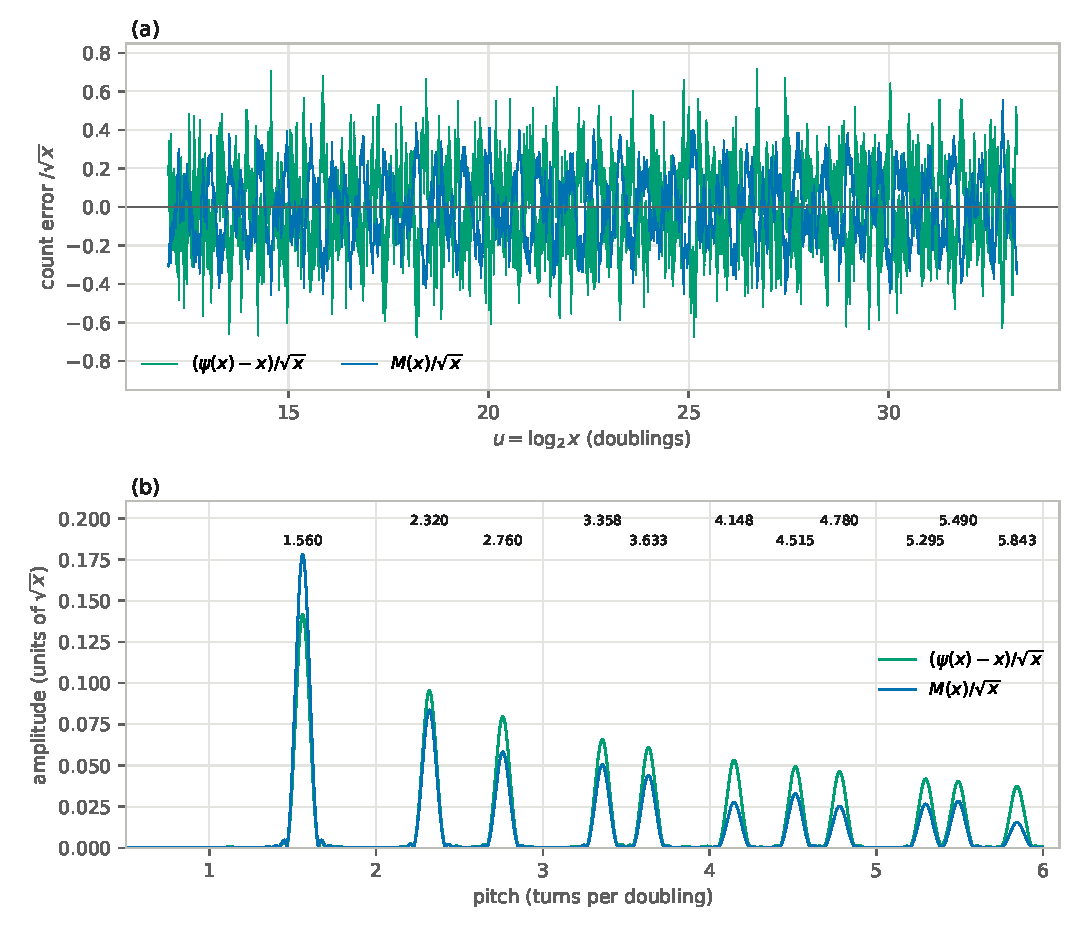
\includegraphics[width=0.93\textwidth]{fig1_waves.pdf}
\caption{(a) $M(x)/\sqrt x$ and $(\psi(x)-x)/\sqrt x$ from exact counts, $2^{12}\le x\le10^{10}$, against $u=\log_2x$. (b) Their spectra in turns per doubling (Hann window over $12\le u\le33.22$), with the peak positions.}\label{fig:waves}
\end{figure}

\begin{table}[h]\centering\small
\begin{tabular}{@{}rrrrrr@{}}\toprule
$k$ & $\gamma_k\log2/2\pi$ & peak, $M$ & peak, $\psi$ & $\delta$, $M$ & $\delta$, $\psi$\\\midrule
1 & 1.5593 & 1.560 & 1.560 & $-0.0003$ & $-0.0006$\\
2 & 2.3191 & 2.320 & 2.320 & $-0.0007$ & $-0.0013$\\
3 & 2.7591 & 2.760 & 2.760 & $-0.0008$ & $+0.0012$\\
4 & 3.3564 & 3.358 & 3.355 & $+0.0003$ & $+0.0001$\\
5 & 3.6333 & 3.633 & 3.633 & $-0.0005$ & $-0.0022$\\
6 & 4.1464 & 4.148 & 4.148 & $-0.0003$ & $+0.0009$\\
7 & 4.5141 & 4.515 & 4.515 & $-0.0018$ & $-0.0013$\\
8 & 4.7797 & 4.780 & 4.780 & $-0.0012$ & $-0.0010$\\\bottomrule
\end{tabular}
\caption{Pitches of the first eight waves from the counts (spectral grid $0.0025$) against $\gamma_k\log2/2\pi$, and the growth exponents $\frac12+\delta$ from the amplitudes over $12\le u\le22.6$ and $22.6\le u\le33.22$.}\label{tab:waves}
\end{table}

\paragraph{Measurement.} From the exact counts at $675{,}247$ checkpoints (\cref{sec:methods}) we interpolate $M(x)$ and $\psi(x)-x$ on the grid $u=12,12.001,\dots,33.219$, divide by $\sqrt x$, and compute the Hann-windowed spectrum on pitches $0.3\le p\le6$ in steps of $0.0025$ (\cref{fig:waves}). The peaks of \cref{tab:waves} coincide with $\gamma_k\log2/2\pi$ to the grid resolution. The means of $M/\sqrt x$ and $(\psi-x)/\sqrt x$ over the range are $-0.0046$ and $-0.0026$. For the growth exponent we compute the amplitude $A_1$ of each wave over $12\le u\le22.6$ and $A_2$ over $22.6\le u\le33.22$ at the pitch $\gamma_k\log2/2\pi$ and put $\delta=\log_2(A_2/A_1)/\Delta u$, $\Delta u=10.6$. The first wave of $(\psi-x)/\sqrt x$ has $A_1=0.1420$ and $A_2=0.1414$, against $2/|\rho_1|=0.14141$ from \cref{lem:real}; that of $M/\sqrt x$ has $A_1=0.1786$ and $A_2=0.1783$. Beyond the eight waves of \cref{tab:waves}, both spectra have peaks at $5.295$, $5.490$ and $5.843$, next to the pitches $5.2958$, $5.4909$ and $5.8436$ of the ninth to eleventh zeros (\cref{fig:waves}b).

\section{The energy}\label{sec:energy}

\begin{proof}[Proof of \cref{mt:energy}]
Suppose RH. By von Koch's theorem \cite{vonKoch} $|\psi(x)-x|\ll\sqrt x\log^2x$, so the integrand of $E$ is $\ll(\log^4x)/x$ and $E(X)\ll\log^5X\ll_\varepsilon X^\varepsilon$.

Conversely, suppose $E(X)\ll_\varepsilon X^\varepsilon$ for every $\varepsilon>0$, and let $\sigma>\frac12$. Choose $0<\varepsilon<2\sigma-1$. For $j\ge0$, by Cauchy--Schwarz,
\begin{align*}
\int_{2^j}^{2^{j+1}}\frac{|\psi(x)-x|}{x^{\sigma+1}}\dd x&=\int_{2^j}^{2^{j+1}}\frac{|\psi(x)-x|}{x}\,x^{-\sigma}\dd x\\
&\le E(2^{j+1})^{1/2}\Bigl(\int_{2^j}^{2^{j+1}}x^{-2\sigma}\dd x\Bigr)^{1/2}\ll2^{j(\varepsilon+1-2\sigma)/2},
\end{align*}
and the sum over $j$ converges. Hence $F(s)=\int_1^\infty(\psi(x)-x)x^{-s-1}\dd x$ converges absolutely and is analytic on $\Re s>\frac12$. For $\Re s>1$, partial summation gives $\int_1^\infty\psi(x)x^{-s-1}\dd x=-\zeta'(s)/(s\zeta(s))$ \cite[Ch.~17]{Davenport}, and $\int_1^\infty x^{-s}\dd x=1/(s-1)$, so
\[
-\frac{\zeta'(s)}{\zeta(s)}=s\Bigl(F(s)+\frac1{s-1}\Bigr).
\]
The right side is meromorphic on $\Re s>\frac12$ with a single pole, at $s=1$. By analytic continuation $\zeta'/\zeta$ has no pole on $\Re s>\frac12$ other than $s=1$, so $\zeta$ has no zero there. By the functional equation there is none on $\Re s<\frac12$ in the critical strip either, and every nontrivial zero lies on the line.

Cramér \cite{Cramer} proved under RH that $\int_2^X(\psi(x)-x)^2x^{-2}\dd x\sim c\log X$, $c=\sum m(\rho)^2|\rho|^{-2}$ over the distinct zeros, and $\int_1^2(\psi(x)-x)^2x^{-2}\dd x=1$. The identity $\sum_\rho\Re(1/\rho)=1+\frac\gamma2-\frac12\log4\pi$ \cite[Ch.~12]{Davenport}, with $1/\rho+1/(1-\rho)=1/(\rho(1-\rho))$ and the symmetries $\rho\mapsto1-\rho$ and $\rho\mapsto\bar\rho$ of the zero set, gives $\sum_\rho1/(\rho(1-\rho))=2+\gamma-\log4\pi$; when $\beta=\frac12$, $\rho(1-\rho)=|\rho|^2$.
\end{proof}

In the variable $u$, $\dd x/x=\log2\dd u$ and $\log X=U\log2$, so $E(2^U)/(U\log2)$ is the mean over $0\le u\le U$ of $((\psi(x)-x)/\sqrt x)^2$. By \cref{lem:real} and the orthogonality of waves of different pitch over long ranges of $u$, the mean square of a sum of waves of constant amplitude $2/|\rho|$, one for each simple zero with $\gamma>0$, is $\sum_{\gamma>0}\frac12(2/|\rho|)^2=\sum_\rho|\rho|^{-2}$: the energy is the sum of the energies of the waves, and it is constant in $u$ exactly when every amplitude is.

\begin{figure}[h]\centering
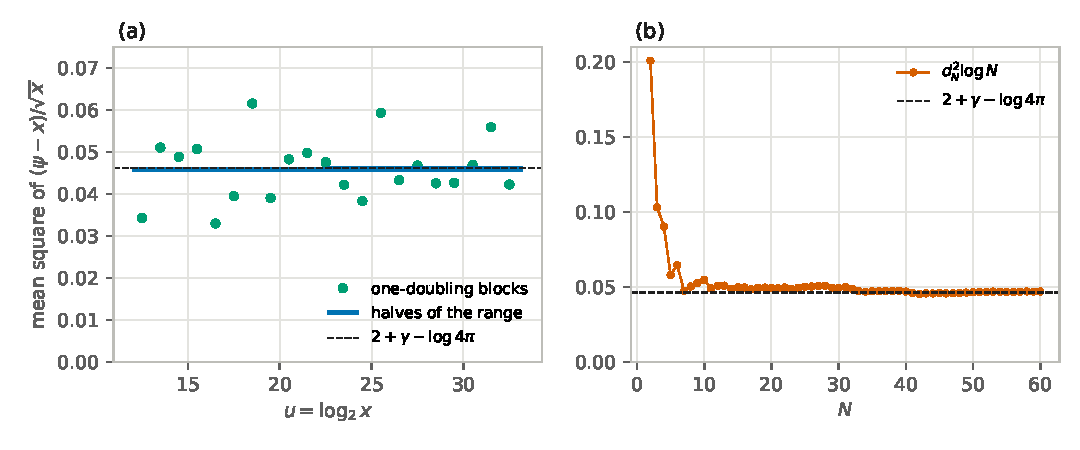
\includegraphics[width=0.95\textwidth]{fig2_energy.pdf}
\caption{(a) The mean of $((\psi(x)-x)/\sqrt x)^2$ over blocks of one doubling and over the two halves of $12\le u\le33.22$, with $2+\gamma-\log4\pi$ (dashed). (b) The sawtooth distance $d_N^2\log N$ for $2\le N\le60$, with the same constant.}\label{fig:energy}
\end{figure}

\paragraph{Measurement.} Over $12\le u\le33.22$ the mean of $((\psi-x)/\sqrt x)^2$ is $0.04592$; over the halves it is $0.04587$ and $0.04597$, and over blocks of one doubling it ranges from $0.033$ to $0.062$, as a finite window of a sum of waves must (\cref{fig:energy}a). Over the $2469$ zeros with $0<\gamma<3000$, all on the line \cite{PT}, $\sum2/(\frac14+\gamma^2)=0.045431$; the zeros above height $T$, counted by the density $\frac1{2\pi}\log\frac t{2\pi}$, add $2\int_T^\infty\frac1{2\pi}\log\frac t{2\pi}\,t^{-2}\dd t=(\log\frac T{2\pi}+1)/(\pi T)=0.000761$ at $T=2999.5$, for a total of $0.046192$ against $2+\gamma-\log4\pi=0.0461914$. The energy measured in the counts to $10^{10}$ is below the energy of the waves by $0.6\%$, and its values in the two halves of the range differ by $0.2\%$.

\section{The sawtooth rebuilds the constant}\label{sec:sawtooth}

Let $\varsigma_k(t)=\fr{1/(kt)}$ and $\chi=\chi_{(0,1]}$, and for $N\ge1$ let
\[
d_N^2=\min_{c\in\R^N}\int_0^\infty\Bigl|\chi(t)-\sum_{k\le N}c_k\varsigma_k(t)\Bigr|^2\dd t .
\]
B\'aez-Duarte \cite{BaezDuarte}, strengthening the criterion of Nyman and Beurling \cite{Beurling}, proved that RH holds if and only if $d_N\to0$. Burnol \cite{Burnol} proved unconditionally that $\liminf_N d_N^2\log N\ge\sum_{\Re\rho=1/2}m(\rho)^2/|\rho|^2$, $m(\rho)$ the multiplicity, and Bettin, Conrey and Farmer \cite{BCF} proved $d_N^2\sim(2+\gamma-\log4\pi)/\log N$ under RH and a hypothesis on $\sum1/|\zeta'(\rho)|^2$. By \cref{mt:countvalue}(a) the weights $c_k=-\mu(k)$ rebuild $\chi$ pointwise; $d_N$ measures how well $N$ sawtooths can do it in mean square.

\begin{lemma}\label{lem:gram}
With $u=1/t$, $\langle\varsigma_j,\varsigma_k\rangle=\int_0^\infty\fr{u/j}\fr{u/k}u^{-2}\dd u$ and $\langle\chi,\varsigma_k\rangle=\int_1^\infty\fr{u/k}u^{-2}\dd u$. On an interval $(a,b)$ on which $\fr{u/j}=u/j-\alpha$ and $\fr{u/k}=u/k-\beta'$ with integers $\alpha,\beta'$,
\[
\int_a^b\frac{\fr{u/j}\fr{u/k}}{u^2}\dd u=\frac{b-a}{jk}-\Bigl(\frac\alpha k+\frac{\beta'}j\Bigr)\log\frac ba+\alpha\beta'\Bigl(\frac1a-\frac1b\Bigr).
\]
Over a period of $\fr{u/j}\fr{u/k}$ the mean is $\frac14+\gcd(j,k)^2/(12jk)$.
\end{lemma}

\begin{proof}
The first two formulas are the substitution $u=1/t$; the third is the integral of $1/(jk)-(\alpha/k+\beta'/j)u^{-1}+\alpha\beta'u^{-2}$. For the mean, write $\fr y=\frac12+B(y)$ with $B(y)=-\sum_{n\ge1}\sin(2\pi ny)/(\pi n)$, so that the mean of $\fr{u/j}\fr{u/k}$ is $\frac14$ plus the mean of $B(u/j)B(u/k)$. With $g=\gcd(j,k)$, $j=gj'$, $k=gk'$, the products of sines have nonzero mean only for $n/j=m/k$, that is $n=j't$, $m=k't$, and the mean is $\sum_{t\ge1}1/(2\pi^2j'k't^2)=1/(12j'k')=g^2/(12jk)$.
\end{proof}

\begin{table}[h]\centering\small
\begin{tabular}{@{}rrr@{\qquad}rrr@{}}\toprule
$N$ & $d_N^2$ & $d_N^2\log N$ & $N$ & $d_N^2$ & $d_N^2\log N$\\\midrule
1 & 0.858212 & -- & 12 & 0.020443 & 0.0508\\
2 & 0.289965 & 0.2010 & 15 & 0.018335 & 0.0497\\
3 & 0.093837 & 0.1031 & 20 & 0.016504 & 0.0494\\
4 & 0.065129 & 0.0903 & 25 & 0.015520 & 0.0500\\
5 & 0.036102 & 0.0581 & 30 & 0.014530 & 0.0494\\
6 & 0.035986 & 0.0645 & 40 & 0.012715 & 0.0469\\
8 & 0.024161 & 0.0502 & 50 & 0.011869 & 0.0464\\
10 & 0.023772 & 0.0547 & 60 & 0.011471 & 0.0470\\\bottomrule
\end{tabular}
\caption{The sawtooth distance from exact integrals of fractional parts.}\label{tab:dN}
\end{table}

\paragraph{Computation.} For $j,k\le60$ we integrate exactly, by \cref{lem:gram}, on $(0,U]$ with $U$ the least multiple of $\mathrm{lcm}(j,k)$ above $4\cdot10^6$, split at the multiples of $j$ and of $k$, and add the tail $\bigl(\frac14+\gcd(j,k)^2/(12jk)\bigr)/U$; the error of the tail is below $\mathrm{lcm}(j,k)/U^2<3\times10^{-10}$. On intervals $(a,b)$ with $a\ge2\cdot10^4$ the closed form of \cref{lem:gram} cancels to many digits, and we use instead its expansion in powers of $1/a$, $jk\int_a^b\fr{u/j}\fr{u/k}u^{-2}\dd u=\int_0^{b-a}(r+\alpha_0)(r+\beta_0)(a+r)^{-2}\dd r=\sum_{n\ge0}(-1)^n(n+1)a^{-n-2}\int_0^{b-a}(r+\alpha_0)(r+\beta_0)r^n\dd r$ with $\alpha_0=j\fr{a/j}$, $\beta_0=k\fr{a/k}$, truncated after seven terms ($(b-a)/a\le3\times10^{-3}$). The inner products $\langle\chi,\varsigma_k\rangle$ are computed in the same way with the tail $\frac12/U$, and agree with the closed form $(\log k+1-\gamma)/k$ to $4\times10^{-13}$. The checks $\langle\varsigma_1,\varsigma_1\rangle=\log2\pi-\gamma=1.2606614015078$ and $\langle\chi,\varsigma_1\rangle=1-\gamma=0.4227843350985$ hold to all $13$ printed digits, and $\langle\varsigma_2,\varsigma_2\rangle=\frac12\langle\varsigma_1,\varsigma_1\rangle$ as the scaling $\varsigma_k(t)=\varsigma_1(kt)$ requires. Then $d_N^2=1-b^{\mathsf T}G^{-1}b$ with $G$ the Gram matrix and $b$ the vector of $\langle\chi,\varsigma_k\rangle$; the condition number of $G$ is $1.3\times10^4$ at $N=60$. \Cref{tab:dN} and \cref{fig:energy}b give the values. For $40\le N\le60$, $d_N^2\log N$ lies between $0.0454$ ($N=42$) and $0.0470$ ($N=58$ and $60$), within $1.8\%$ of $2+\gamma-\log4\pi=0.0461914$, and crosses it between $N=48$ and $N=49$: the distance by which $N$ sawtooths of the exact count fall short of the constant, per unit of $1/\log N$, agrees in this range with the energy per unit of $\log x$ of the prime count's error in \cref{sec:energy}, and under RH and the hypothesis of \cite{BCF} the two are equal in the limit.

\section{The rebuild law beyond \texorpdfstring{$10^{10}$}{10\^{}10}}\label{sec:beyond}

With a table of $\mu$ to $L=10^9$, built by the pairing (each prime flips the sign of its multiples and each prime square annihilates them), \cref{rem:recursion} evaluates $M(x)$ from the law and the table. It returns $M(10^9)=-222$, $M(10^{10})=-33{,}722$, $M(10^{11})=-87{,}856$, $M(10^{12})=62{,}366$, $M(10^{13})=599{,}582$, $M(10^{14})=-875{,}575$ and $M(10^{15})=-3{,}216{,}373$, the published values \cite{OEISM}; $M(10^{10})$ also agrees with our sieve. \Cref{tab:doublings} gives the doublings, which agree with \cite{OEISM2}.

\begin{table}[h]\centering\small
\begin{tabular}{@{}rrr@{\qquad}rrr@{}}\toprule
$x$ & $M(x)$ & $M/\sqrt x$ & $x$ & $M(x)$ & $M/\sqrt x$\\\midrule
$2^{34}$ & $-3{,}421$ & $-0.026$ & $2^{42}$ & $-169{,}338$ & $-0.081$\\
$2^{35}$ & $8{,}435$ & $0.046$ & $2^{43}$ & $259{,}886$ & $0.088$\\
$2^{36}$ & $38{,}176$ & $0.146$ & $2^{44}$ & $-474{,}483$ & $-0.113$\\
$2^{37}$ & $-28{,}118$ & $-0.076$ & $2^{45}$ & $1{,}726{,}370$ & $0.291$\\
$2^{38}$ & $38{,}729$ & $0.074$ & $2^{46}$ & $-3{,}554{,}573$ & $-0.424$\\
$2^{39}$ & $-135{,}944$ & $-0.183$ & $2^{47}$ & $-135{,}443$ & $-0.011$\\
$2^{40}$ & $101{,}597$ & $0.097$ & $2^{48}$ & $3{,}282{,}200$ & $0.196$\\
$2^{41}$ & $15{,}295$ & $0.010$ & $2^{49}$ & $1{,}958{,}235$ & $0.083$\\\bottomrule
\end{tabular}
\caption{$M(x)$ from the rebuild law at the doublings $2^{34}$ to $2^{49}$.}\label{tab:doublings}
\end{table}

At $10^{11},\dots,10^{15}$ the ratio $M/\sqrt x$ is $-0.278$, $0.062$, $0.190$, $-0.088$ and $-0.102$. Over all the points evaluated the largest value of $|M|/\sqrt x$ is $0.424$, at $2^{46}$.

\section{The small primes and the newest primes}\label{sec:small}

\paragraph{The integers free of the primes up to 37.} Let $P=\prod_{p\le37}p$ and $\Phi_{37}(x)=\#\{n\le x:(n,P)=1\}=\sum_{d\mid P}\mu(d)\lfloor x/d\rfloor$. Then $\Phi_{37}(x)-x\prod_{p\le37}(1-1/p)=-\sum_{d\mid P}\mu(d)\fr{x/d}$ is bounded by $2^{11}$ and periodic with period $P$. Evaluated exactly on the grid of \cref{sec:waves}, its absolute value is at most $38.9$ for $2^{12}\le x\le10^{10}$, and at $x=10^{10}$ it is $18.4=0.00018\sqrt x$; its spectrum in doublings has amplitude at most $0.0018$ at every pitch in $[0.3,6]$, and at most $0.0017$ at the pitches of \cref{tab:waves}, against $0.14$--$0.18$ for the first wave of the prime counts. Of the $1{,}487{,}210{,}140$ integers up to $10^{10}$ that it counts, $455{,}052{,}499$ are prime. Since the primes up to $37$ contribute $O(\log x)$ to $\psi(x)$ and the sieve by them leaves an error bounded by $2^{11}$, the waves of \cref{sec:waves} lie in the placement of the primes above $37$ among the integers free of the primes up to $37$.

\paragraph{The newest primes.} Let $M(x,y)=\sum_{n\le x,\,P^+(n)\le y}\mu(n)$, $P^+(n)$ the largest prime factor. An integer $n\le x$ with $P^+(n)=p>x/2$ is $n=p$, so
\[
M(x)=M(x,x/2)-\bigl(\pi(x)-\pi(x/2)\bigr).
\]
At $x=10^{10}$, $\pi(x)=455{,}052{,}511$, $\pi(x/2)=234{,}954{,}223$ and $M(x)=-33{,}722$, so $M(x,x/2)=220{,}064{,}566=2200.6\sqrt x$: the primes in $(x/2,x]$ bring the balance from $2200.6\sqrt x$ to $-0.337\sqrt x$. The sieve also gives $M(x,\sqrt x)=-219.4\sqrt x$ at $x=10^{10}$. At $x=10^{10}$ the sum reaches the scale $\sqrt x$ only when the primes in $(x/2,x]$ are included.

\paragraph{A sign that holds for $9\times10^8$ steps.} The sum $L(x)$ of the Liouville function satisfies $L(x)\le0$ for $2\le x<906{,}150{,}257$ and $L(906{,}150{,}257)=1$ \cite{Tanaka}, which our sieve confirms.

\begin{remark}[the count must be exact]\label{rem:exact}
In the system of \cref{mt:beurling} and in the systems of \cite{BDR} the pairing of \cref{mt:rebuild}(i) holds, because factorisation into generalized primes is unique, and so does the rebuild law over the generalized integers. In the system of \cref{mt:beurling}, and in the systems of \cite{BDR} with $\alpha>\frac23$ below, the energy $E_B(X)=\int_1^X((\psi_B(x)-x)/x)^2\dd x$ exceeds a fixed positive power of $X$ for arbitrarily large $X$. Indeed $\psi_B$ is nondecreasing, so if $0<h\le x_0$ and $\psi_B(x_0)-x_0\ge h$, then $\psi_B(x)-x\ge h/2$ on $[x_0,x_0+h/2]$, and if $\psi_B(x_0)-x_0\le-h$, then $\psi_B(x)-x\le-h/2$ on $[x_0-h/2,x_0]$; either interval contributes at least $h^3/(18x_0^2)$ to $E_B(2x_0)$. With $h=x_0^{\alpha'}$ this is $x_0^{3\alpha'-2}/18$. In the system of \cref{mt:beurling}, let $\frac12<\alpha'<1$. If $\psi_B(x)-x=O(x^{\alpha'})$, then, since the prime powers $p^k\le x$ with $k\ge2$ contribute $O(\sqrt x\log x)$ to $\psi_B(x)$, the sum $\theta_B(x)$ of $\log p$ over the generalized primes $p\le x$ satisfies $\theta_B(x)-x=O(x^{\alpha'})$, and partial summation gives $\pi_B(x)-\mathrm{li}(x)=O(x^{\alpha'})$, contrary to $\pi_B(x)-\mathrm{li}(x)=\Omega(x\exp(-c\sqrt{\log x}))$; so $|\psi_B(x)-x|\ge x^{\alpha'}$ for arbitrarily large $x$. Broucke, Debruyne and R\'ev\'esz \cite{BDR} construct, for each $\alpha\in[0,1)$ and $\beta\in[\frac12,1)$, systems with $\psi_B(x)=x+O(x^{\alpha+\varepsilon})$ and $N_B(x)=\kappa x+O(x^{\beta+\varepsilon})$ for every $\varepsilon>0$, neither exponent being improvable; with $\beta=\frac12$ and $\alpha>\frac23$, $|\psi_B(x)-x|\ge x^{\alpha'}$ for arbitrarily large $x$ whenever $\alpha'<\alpha$, and taking $\frac23<\alpha'<\alpha$ the energy exceeds a power of $X$ for arbitrarily large $X$. An argument that derived \cref{conj:energy} from the pairing, the rebuild law and a bound $O(x^{1/2+\varepsilon})$ for the error of the integer count would apply to these systems as well, where its conclusion is false. For the ordinary integers the error of the count is $-\fr x$, bounded by $1$, and this is what $d_N$ measures: the sawtooths $\varsigma_k$ are the errors of the counts $\lfloor1/(kt)\rfloor$.
\end{remark}

\section{Methods of computation}\label{sec:methods}

\paragraph{Counts to $10^{10}$.} An exact segmented sieve to $10^{10}$ gives $\mu(n)$, $\lambda(n)$ and $\Lambda(n)$ and records $M$, $L$, $\pi$ and $\psi-x$ in extended precision at $675{,}247$ checkpoints; at the top of the range consecutive checkpoints differ by $3.3\times10^{-4}$ in $\log_2x$. It returns $\pi(10^{10})=455{,}052{,}511$, $M(10^{10})=-33{,}722$ and $L(10^{10})=-116{,}026$.

\paragraph{The rebuild law.} \Cref{rem:recursion} in 64-bit integer arithmetic with $L=10^9$; $M(10^{15})$ takes about $10^{11}$ integer divisions.

\paragraph{Spectra and energy.} Linear interpolation of the checkpoint values on the grid $\Delta u=10^{-3}$, Hann window, direct evaluation of the Fourier sum at each pitch.

\paragraph{Zeros.} The $2469$ zeros of $\zeta$ with $0<\gamma<3000$ are the sign changes of Hardy's function $Z(t)$, evaluated by Euler--Maclaurin summation on a grid of one twelfth of the mean spacing and refined by Brent's method to $10^{-13}$ \cite{S09}; an independent evaluation of $Z$ by the Riemann--Siegel formula gives the same $2469$ sign changes and the same $\sum2/(\frac14+\gamma^2)$ to six digits. All lie on the critical line \cite{PT}.

\paragraph{Sawtooth integrals.} \Cref{lem:gram} in double precision; the linear systems by Gaussian elimination.

\paragraph{The count of \cref{sec:small}.} Inclusion--exclusion over the $4096$ squarefree divisors of $\prod_{p\le37}p$ in exact integer arithmetic.

\section{Concluding remarks}\label{sec:concl}

\paragraph{What the paper fixes about the remaining step.} The pairing makes the rebuild law hold, and the law fixes the balance at every scale from the smaller ones (\cref{mt:rebuild}); the pair-weighted sawtooths rebuild the constant exactly, and every finite rebuild falls short by the value imbalance and by the unfinished pairs (\cref{mt:countvalue}); RH is the subpolynomial growth of the energy of the count's error (\cref{mt:energy}), and the energy measured in the counts, the energy of the waves and the sawtooth distance per unit of $1/\log N$ agree with the single constant $2+\gamma-\log4\pi$ to within $2\%$. The pairing and the law hold in Beurling systems whose energy exceeds a power of $X$ for arbitrarily large $X$ (\cref{rem:exact}), so the step must use more about the count than these; the ordinary count is exact.

\paragraph{Outlook.} The next computations are the energy of $M$ and of $\psi$ in doublings beyond $10^{10}$, from the rebuild law and its analogue for $\psi$, and $d_N$ for $N$ in the thousands by the same exact integrals. The next analytic question is how the exactness of the count, the bound $|\fr x|<1$ that no Beurling system with a power-size error shares, enters a bound for $E(X)$.

\section{Data and sources}\label{sec:data}
\paragraph{External inputs.} All inputs are mathematical; no measured data are used.
\begin{enumerate}[label=(\roman*)]
\item All nontrivial zeros of $\zeta$ with $0<\gamma\le3\cdot10^{12}$ lie on the critical line \cite{PT}.
\item Published values used for comparison: $M(10^n)$, $n\le15$ \cite{OEISM}; $M(2^n)$, $34\le n\le49$ \cite{OEISM2}; $\pi(10^{10})=455{,}052{,}511$ \cite{OEISpi}; the least $x>1$ with $L(x)>0$, $906{,}150{,}257$ \cite{Tanaka}.
\item Classical and published theorems: Littlewood's criterion \cite[\S14.25]{Titchmarsh}; von Koch's bound \cite{vonKoch}; Cramér's mean value theorem \cite{Cramer}; the explicit formula and $\sum_\rho\Re(1/\rho)$ \cite{Davenport}; $\sum\mu(k)/k=0$ \cite{Apostol}; the criterion of Nyman, Beurling and B\'aez-Duarte \cite{Beurling,BaezDuarte}; Burnol's bound \cite{Burnol}; the asymptotic of Bettin, Conrey and Farmer \cite{BCF}; the Beurling systems of \cite{DMV,BDR}; the closed forms of the Gram integrals \cite{Vasyunin} and the earlier computations of $d_N$ \cite{LandreauRichard}; $\limsup|M(x)|/\sqrt x>1$ \cite{OdlyzkoTeRiele}.
\end{enumerate}
\paragraph{Computed quantities.} Every other number in the paper is computed from formulas stated in the text by the methods of \cref{sec:methods}: the counts to $10^{10}$, the spectra, growth exponents and energies, the sums over zeros, the Gram matrices and $d_N$, the values of $M$ from the rebuild law to $10^{15}$, $m(N)$ to $10^8$, and the count of integers free of the primes up to $37$.


\begin{thebibliography}{99}\small
\bibitem{Apostol} T.~M.~Apostol, \emph{Introduction to Analytic Number Theory}, Undergraduate Texts in Mathematics, Springer, New York, 1976.
\bibitem{BaezDuarte} L.~B\'aez-Duarte, A strengthening of the Nyman--Beurling criterion for the Riemann hypothesis, \emph{Atti Accad. Naz. Lincei Rend. Lincei Mat. Appl.} 14 (2003) 5--11.
\bibitem{BCF} S.~Bettin, J.~B.~Conrey, D.~W.~Farmer, An optimal choice of Dirichlet polynomials for the Nyman--Beurling criterion, \emph{Proc. Steklov Inst. Math.} 280, suppl.~2 (2013) S30--S36.
\bibitem{Beurling} A.~Beurling, A closure problem related to the Riemann zeta-function, \emph{Proc. Nat. Acad. Sci. U.S.A.} 41 (1955) 312--314.
\bibitem{BDR} F.~Broucke, G.~Debruyne, Sz.~Gy.~R\'ev\'esz, Some examples of well-behaved Beurling number systems, \emph{Trans. Amer. Math. Soc.} 378 (2025) 477--501.
\bibitem{Burnol} J.-F.~Burnol, A lower bound in an approximation problem involving the zeros of the Riemann zeta function, \emph{Adv. Math.} 170 (2002) 56--70.
\bibitem{Cramer} H.~Cram\'er, Ein Mittelwertsatz in der Primzahltheorie, \emph{Math. Z.} 12 (1922) 147--153.
\bibitem{LandreauRichard} B.~Landreau, F.~Richard, Le crit\`ere de Beurling et Nyman pour l'hypoth\`ese de Riemann: aspects num\'eriques, \emph{Experiment. Math.} 11 (2002) 349--360.
\bibitem{Davenport} H.~Davenport, \emph{Multiplicative Number Theory}, 3rd ed., revised by H.~L.~Montgomery, Graduate Texts in Mathematics 74, Springer, New York, 2000.
\bibitem{DMV} H.~G.~Diamond, H.~L.~Montgomery, U.~M.~A.~Vorhauer, Beurling primes with large oscillation, \emph{Math. Ann.} 334 (2006) 1--36.
\bibitem{OdlyzkoTeRiele} A.~M.~Odlyzko, H.~J.~J.~te Riele, Disproof of the Mertens conjecture, \emph{J. Reine Angew. Math.} 357 (1985) 138--160.
\bibitem{OEISpi} OEIS Foundation, Sequence A006880, number of primes $<10^n$, \emph{The On-Line Encyclopedia of Integer Sequences}, \url{https://oeis.org/A006880} (accessed 25 September 2026).
\bibitem{OEISM} OEIS Foundation, Sequence A084237, $a(n)=M(10^n)$, where $M(n)$ is Mertens's function, \emph{The On-Line Encyclopedia of Integer Sequences}, \url{https://oeis.org/A084237} (accessed 26 September 2026).
\bibitem{OEISM2} OEIS Foundation, Sequence A084236, $a(n)=M(2^n)$, where $M(n)$ is Mertens's function, \emph{The On-Line Encyclopedia of Integer Sequences}, \url{https://oeis.org/A084236} (accessed 26 September 2026).
\bibitem{PT} D.~Platt, T.~Trudgian, The Riemann hypothesis is true up to $3\cdot10^{12}$, \emph{Bull. London Math. Soc.} 53 (2021) 792--797.
\bibitem{S09} A.~Singh, The Remaining Step: Six Equivalent Forms of the Riemann Hypothesis and the Surgery Obstruction, manuscript, 25 September 2026.
\bibitem{Tanaka} M.~Tanaka, A numerical investigation on cumulative sum of the Liouville function, \emph{Tokyo J. Math.} 3 (1980) 187--189.
\bibitem{Titchmarsh} E.~C.~Titchmarsh, \emph{The Theory of the Riemann Zeta-Function}, 2nd ed., revised by D.~R.~Heath-Brown, Oxford University Press, Oxford, 1986.
\bibitem{Vasyunin} V.~I.~Vasyunin, On a biorthogonal system associated with the Riemann hypothesis, \emph{St. Petersburg Math. J.} 7 (1996) 405--419.
\bibitem{vonKoch} H.~von Koch, Sur la distribution des nombres premiers, \emph{Acta Math.} 24 (1901) 159--182.
\end{thebibliography}
\end{document}
